% Gemini theme
% Author: Lukas Hölsch

\documentclass[final]{beamer}

% ====================
% Packages
% ====================

% \usepackage[T1]{fontenc}
% \usepackage{lmodern}
\usepackage[size=a0,orientation=landscape,scale=1.0]{beamerposter}
\usetheme{gemini}
\usecolortheme{unisiegen}
\usepackage{graphicx}
\usepackage{booktabs}
\usepackage{tikz}
\usepackage{pgfplots}
\pgfplotsset{compat=1.14}
% \usepackage{anyfontsize}
\usepackage{qrcode}
\usepackage{caption}
\usepackage{wrapfig}
\usepackage{bm}
\usepackage{multirow}
\usepackage{fancyqr}
\usepackage{fontawesome5}
\usepackage{subcaption}
% \usepackage{amsfonts}
% \usepackage[cm]{sfmath}

% ====================
% Lengths
% ====================

% If you have N columns, choose \sepwidth and \colwidth such that
% (N+1)*\sepwidth + N*\colwidth = \paperwidth
\newlength{\sepwidth}
\newlength{\colwidth}
\setlength{\sepwidth}{0.025\paperwidth}
\setlength{\colwidth}{0.3\paperwidth}

\newcommand{\separatorcolumn}{\begin{column}{\sepwidth}\end{column}}

% ====================
% Title
% ====================

\title{Calculation of Optimized Pulse Patterns for Electric Drives with an End-To-End Differentiable Simulation Framework}

\author{Lukas Hölsch \inst{1}, Daniel Wiechmann \inst{1}, Oliver Schweins \inst{2}, Oliver Wallscheid \inst{1}}

\institute[shortinst]{\inst{1} Chair of Interconnected Automation Systems, University of Siegen, Germany \samelineand \inst{2} Power Electronics and Electrical Drives, Paderborn University, Germany}

% ====================
% Footer (optional)
% ====================

\footercontent{
  \href{https://www.uni-siegen.de/ias}{https://www.uni-siegen.de/ias} \hfill
  IEMDC 2025, Houston \hfill
  \href{mailto:lukas.hoelsch@uni-siegen.de}{lukas.hoelsch@uni-siegen.de}}
% (can be left out to remove footer)

% ====================
% Logo (optional)
% ====================

% use this to include logos on the left and/or right side of the header:
% \logoright{
\includegraphics[height=4cm]{assets/UNIS-Dachmarke_kurz_rgb_unis_dachmarke.svg}}
\logoleft{
\includegraphics[height=7cm]{assets/UNIS-Dachmarke_cmyk.pdf}}

% ====================
% Body
% ====================

\begin{document}

\begin{frame}[t]
  \begin{columns}[t]
    \separatorcolumn
    \begin{column}{\colwidth}

      %%%%%%%%%%%%%%%%%%%%%%%%%%%%%%%%%%%%%%%%%%%%%%
      %% Simulation framework
      %%%%%%%%%%%%%%%%%%%%%%%%%%%%%%%%%%%%%%%%%%%%%%
      \begin{block}{Simulation framework}
        \begin{figure}[htb]
          \centering
          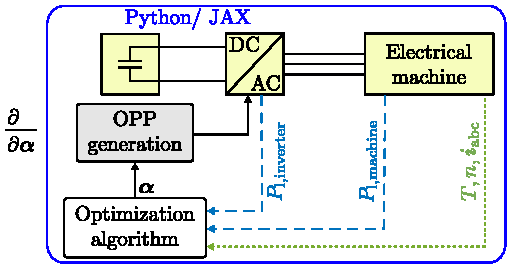
\includegraphics[width=0.7\textwidth]{fig/simulation_structure.pdf}
          \caption{End-to-end differentiable simulation framework.}
          \label{fig:simulation_framework}
        \end{figure}
      \end{block}

      %%%%%%%%%%%%%%%%%%%%%%%%%%%%%%%%%%%%%%%%%%%%%%
      %% Contribution
      %%%%%%%%%%%%%%%%%%%%%%%%%%%%%%%%%%%%%%%%%%%%%%
      \begin{alertblock}{Contribution}
        \begin{itemize}
          \item End-to-end differentiable simulation to calculate OPPs
          \item Utilization of the nonlinear machine model
          \item Considering the inverter and machine losses in the cost function
        \end{itemize}
      \end{alertblock}

      %%%%%%%%%%%%%%%%%%%%%%%%%%%%%%%%%%%%%%%%%%%%%%
      %% Flux linkage
      %%%%%%%%%%%%%%%%%%%%%%%%%%%%%%%%%%%%%%%%%%%%%%
      % \begin{block}{Nonlinear flux linkage mpas}

      %   Measured flux linkage maps at the test bench at a fixed speed.
      %   \begin{figure}[htb]
      %     \centering
      %     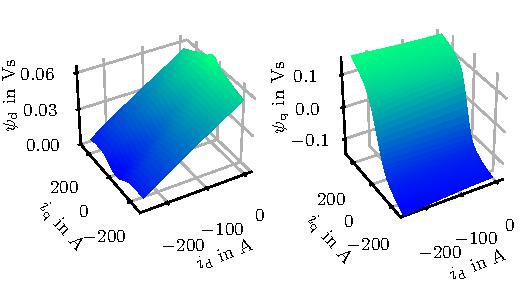
\includegraphics[width=0.7\textwidth]{fig/fluxLinkage.pdf}
      %     \caption{Nonlinear flux linkage maps of the utilized PMSM.}
      %     \label{fig:fluxLinkage}
      %   \end{figure}
      % \end{block}

      %%%%%%%%%%%%%%%%%%%%%%%%%%%%%%%%%%%%%%%%%%%%%%
      %% Differential inductances
      %%%%%%%%%%%%%%%%%%%%%%%%%%%%%%%%%%%%%%%%%%%%%%
      \begin{block}{Differential inductances}
        \begin{figure}[htb]
          \centering
          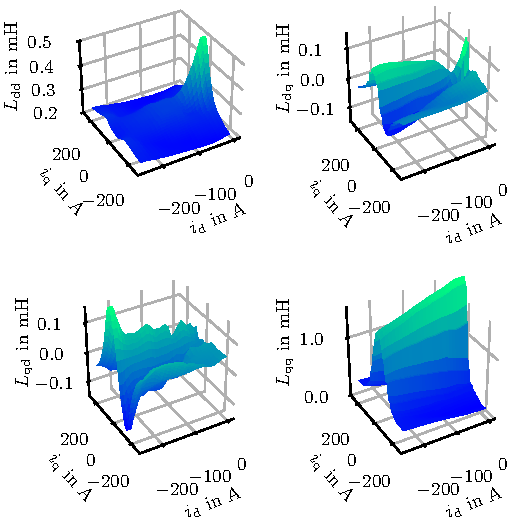
\includegraphics[width=0.65\textwidth]{fig/diffInductances.pdf}
          \caption{Differential inductances of the utilized PMSM.}
          \label{fig:diffInductances}
        \end{figure}
      \end{block}

      %%%%%%%%%%%%%%%%%%%%%%%%%%%%%%%%%%%%%%%%%%%%
      %% Modulation index
      %%%%%%%%%%%%%%%%%%%%%%%%%%%%%%%%%%%%%%%%%%%%
      \begin{block}{Modulation index}
        \begin{figure}[htb]
          \centering
          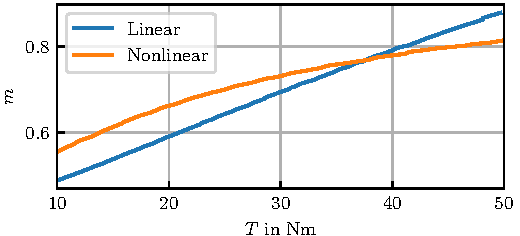
\includegraphics[width=0.65\textwidth]{fig/modulation_index.pdf}
          \caption{Comparison of the modulation index for the linear and nonlinear PMSM model.}
          \label{fig:modulation_idx}
        \end{figure}
      \end{block}

    \end{column}

    %%%%%%%%%%%%%%%%%%%%%%%%%%%%%%%%%%%%%%%%%%%%
    %% Second column
    %%%%%%%%%%%%%%%%%%%%%%%%%%%%%%%%%%%%%%%%%%%%
    \separatorcolumn
    \begin{column}{\colwidth}

      %%%%%%%%%%%%%%%%%%%%%%%%%%%%%%%%%%%%%%%%%%%%%%%
      %% Cost function
      %%%%%%%%%%%%%%%%%%%%%%%%%%%%%%%%%%%%%%%%%%%%%%%
      \begin{alertblock}{Cost function}
        \begin{subequations}
          \begin{equation*}
            \underset{\bm{\alpha}}{\mathrm{min}}  \ J = k_{\mathrm{l,inv}} P_{\mathrm{l,inverter}} + k_{\mathrm{l,mach}} P_{\mathrm{l,machine}}
          \end{equation*}
          \begin{equation*}
            \mathrm{s.t.} \hspace{5mm} \frac{\mathrm{d}}{\mathrm{d}t}\bm{x}=\bm{f}(\bm{x},\bm{u}), \hspace{5mm} \overline{T}=T^*
          \end{equation*}
          \begin{equation*}
            \hspace{20mm} 0 \le \alpha_1 \le ... \le \alpha_M \le \frac{\pi}{2}
          \end{equation*}
        \end{subequations}
      \end{alertblock}

      %%%%%%%%%%%%%%%%%%%%%%%%%%%%%%%%%%%%%%%%%%%%
      %% Pulse pattern
      %%%%%%%%%%%%%%%%%%%%%%%%%%%%%%%%%%%%%%%%%%%%
      \begin{block}{Pulse pattern}
        \begin{figure}[htb]
          \centering
          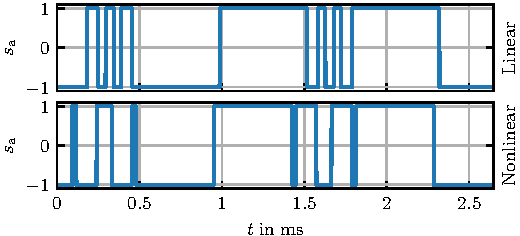
\includegraphics[width=0.7\textwidth]{fig/OPP_lin_nonlin.pdf}
          \caption{Corresponding pulse patterns to the current trajectories in Fig.\ref{fig:i_ab_cross_check}.}
          \label{fig:OPP_lin_nonlin}
        \end{figure}
      \end{block}

      %%%%%%%%%%%%%%%%%%%%%%%%%%%%%%%%%%%%%%%%%%%%
      %% Stator current
      %%%%%%%%%%%%%%%%%%%%%%%%%%%%%%%%%%%%%%%%%%%%
      \begin{block}{Stator current}
        \begin{figure}[htb]
          \centering
          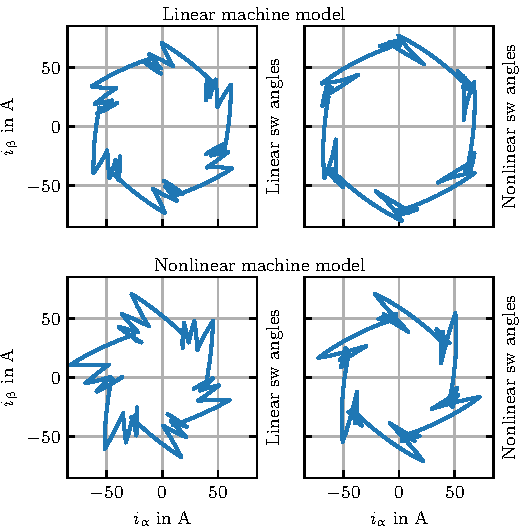
\includegraphics[width=0.7\textwidth]{fig/i_ab_cross_check.pdf}
          \caption{Current trajectories for one operating point to highlight the difference between the linear and nonlinear PMSM model.}
          \label{fig:i_ab_cross_check}
        \end{figure}
      \end{block}

      \vspace{1cm}

      %%%%%%%%%%%%%%%%%%%%%%%%%%%%%%%%%%%%%%%%%%%%
      %% Specification of the operating points
      %%%%%%%%%%%%%%%%%%%%%%%%%%%%%%%%%%%%%%%%%%%%
      % \begin{block}{Specification of the operating points}
      \begin{table}[ht]
        \caption{Specification of the operating points.}
        \centering
        \begin{tabular}{lr}\toprule
          $T^* \in \left[10,40\right]$~Nm           \\
          $n^* = 7750~\mathrm{\min}^{-1}$           \\
          Number of initial start angles      & 500 \\
          Iterations optimizer per evaluation & 100 \\
          \bottomrule
        \end{tabular}
        \label{tab:operating_point_simulations}
      \end{table}
      % \end{block}

    \end{column}

    %%%%%%%%%%%%%%%%%%%%%%%%%%%%%%%%%%%%%%%%%
    %% third column
    %%%%%%%%%%%%%%%%%%%%%%%%%%%%%%%%%%%%%%%%%
    \separatorcolumn
    \begin{column}{\colwidth}

      %%%%%%%%%%%%%%%%%%%%%%%%%%%%%%%%%%%%%%%%%%%%
      %% Computational effort of the optimization
      %%%%%%%%%%%%%%%%%%%%%%%%%%%%%%%%%%%%%%%%%%%%
      % \begin{block}{Computational effort of the optimization}
      \begin{table}[ht]
        \caption{Computational effort of the optimization for one operating point (OPP3). The simulations are performed on the CPU of a workstation (AMD Ryzen 9 5950X @3.4 GHz) with 16 cores.}
        \centering
        \begin{tabular}{lcc}\toprule
          \multirow{2}{*}{OPP3}            & \multicolumn{2}{c}{Machine model}             \\
                                           & Linear                            & Nonlinear \\
          \midrule
          Trials                           & 90                                & 70        \\
          Average time per operating point & 5.27 min                          & 28.07 min \\
          95th percentile time             & 5.29 min                          & 29.10 min \\
          \bottomrule
        \end{tabular}
        \label{tab:computational_effort}
      \end{table}
      % \end{block}

      %%%%%%%%%%%%%%%%%%%%%%%%%%%%%%%%%%%%%%%%%%%%
      %% Switching angles
      %%%%%%%%%%%%%%%%%%%%%%%%%%%%%%%%%%%%%%%%%%%%
      \begin{block}{Switching angles}
        \begin{figure}[htb]
          \centering
          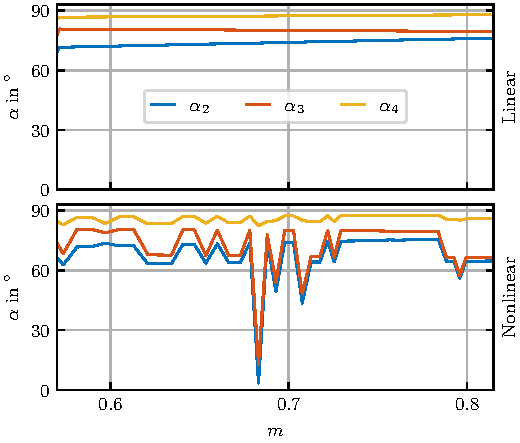
\includegraphics[width=0.65\textwidth]{fig/sw_angles.pdf}
          \caption{Comparison of the switching angles between a linear and nonlinear PMSM model for a fix rotational speed of $n=7500~\mathrm{\min}^{-1}$ and $T^* \in \left[10, 50\right] \ \mathrm{Nm}$.}
          \label{fig:sw_angles}
        \end{figure}
      \end{block}

      %%%%%%%%%%%%%%%%%%%%%%%%%%%%%%%%%%%%%%%%%%%%%%
      %% Loss evaluation
      %%%%%%%%%%%%%%%%%%%%%%%%%%%%%%%%%%%%%%%%%%%%%%
      % \begin{block}{Loss evaluation}
      %   \begin{figure}[htb]
      %     \centering
      %     \includegraphics[width=0.7\textwidth]{fig/losses.pdf}
      %     \caption{Evaluation of the total losses for the nonlinear PMSM model in the top part, where the separated losses are shown in the figure below. The influence of the average switching frequency due to the pulse pattern candidate is shown.}
      %     \label{fig:losses}
      %   \end{figure}
      % \end{block}

      %%%%%%%%%%%%%%%%%%%%%%%%%%%%%%%%%%%%%%%%%%%%
      %% Multi objective optimization
      %%%%%%%%%%%%%%%%%%%%%%%%%%%%%%%%%%%%%%%%%%%%
      \begin{block}{Multi-objective optimization}
        \begin{figure}[htb]
          \centering
          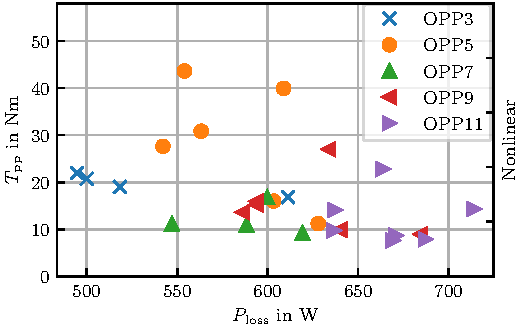
\includegraphics[width=0.65\textwidth]{fig/paretoFront.pdf}
          \caption{Pareto plane for one specific operating point with $n=7500~\mathrm{\min}^{-1}$ and $T^* = 40 \ \mathrm{Nm}$. Much more simulations have been carried out as depicted in the figure. However, they result in the same minima.}
          \label{fig:paretoFront}
        \end{figure}
      \end{block}

      %%%%%%%%%%%%%%%%%%%%%%%%%%%%%%%%%%%%%%%%%%%%
      %% Evaluation
      %%%%%%%%%%%%%%%%%%%%%%%%%%%%%%%%%%%%%%%%%%%%
      % \begin{block}{Evaluation}
      %   \begin{figure}[htb]
      %     \centering
      %     \includegraphics[width=0.7\textwidth]{fig/OPP7_PWM7.pdf}
      %     \caption{Loss and torque ripple comparison between an OPP7 and a triangular carrier-based PWM.}
      %     \label{fig:OPP7_PWM7}
      %   \end{figure}
      % \end{block}

      %%%%%%%%%%%%%%%%%%%%%%%%%%%%%%%%%%%%%%%%%%%%
      %% Conclusion
      %%%%%%%%%%%%%%%%%%%%%%%%%%%%%%%%%%%%%%%%%%%%
      \begin{alertblock}{Conclusion}
        \begin{itemize}
          % \item Python with JAX library for electric drives
          \item Highlight the difference between the linear and nonlinear machine model by comparison of the stator current trajectories
          \item Reducing the electric drive losses of approx. 8\,\% and torque ripple of 39\,\%
        \end{itemize}
      \end{alertblock}

      %%%%%%%%%%%%%%%%%%%%%%%%%%%%%%%%%%%%%%%%%%%%
      %% Outlook
      %%%%%%%%%%%%%%%%%%%%%%%%%%%%%%%%%%%%%%%%%%%%
      % \begin{alertblock}{Outlook}
      %   \begin{itemize}
      %     \item Adaptive step size to reduce the computational effort
      %     \item Improvement of the cost function, e.g., consideration of interlocking times
      %   \end{itemize}
      % \end{alertblock}

      %%%%%%%%%%%%%%%%%%%%%%%%%%%%%%%%%%%%%%%%%%%%
      %% Contact
      %%%%%%%%%%%%%%%%%%%%%%%%%%%%%%%%%%%%%%%%%%%%
      \begin{block}{Contact}
        \begin{figure}[ht]
          \centering
          \begin{minipage}{0.15\textwidth}
            \fancyqr[image = {\includegraphics[width=1.1cm]{assets/UNIS-Dachmarke_kurz_PAT.pdf}}, image padding=1, height=4cm, color=unidarkblue, level=H]{https://www.uni-siegen.de/ias}
          \end{minipage}%
          \begin{minipage}{0.34\textwidth}
            Lukas Hölsch\\
            lukas.hoelsch@uni-siegen.de
          \end{minipage}
          \hspace{4cm}
          \begin{minipage}{0.15\textwidth}
            \fancyqr[image = {\color{unidarkblue} \large \faGithub}, image padding=1, height=4cm, color=unidarkblue, level=H]{https://www.github.com/orgs/IAS-Uni-Siegen}
          \end{minipage}%
          \begin{minipage}{0.15\textwidth}
            IAS GitHub
          \end{minipage}
        \end{figure}
      \end{block}

    \end{column}
    \separatorcolumn
  \end{columns}
\end{frame}

\end{document}